%%%%%%%%%%%%%%%%%%%%%%%%%%%%%%%%%%%%%%%%%%%%%%%%%%%%%%%%%%%%%%%%%%%%%%%%%%%%%%%%

\begin{solution}
\begin{enumerate}
\item {[5 points]} Since $f(x) = x^2(1-x) = x^2-x^3$, we have that, for $k=1,2,\ldots$,
\begin{eqnarray*}
(f,\psi_k)&=&\sqrt{2}\int_0^1 \left(x^2-x^3\right) \sin\left(k\pi x\right)\, dx
\\
&=&\sqrt{2}\left(\left[-{1\over k\pi}\left(x^2-x^3\right)\cos\left(k\pi x\right)\right]_0^1+{1\over k\pi}\int_0^1 \left(2x-3x^2\right) \cos(k\pi x)\, dx\right)
\\
&=&{\sqrt{2}\over k\pi}\int_0^1 \left(2x-3x^2\right) \cos(k\pi x)\, dx
\\
&=&{\sqrt{2}\over k\pi}\left(\left[{1\over k\pi}\left(2x-3x^2\right)\sin\left(k\pi x\right)\right]_0^1-{1\over k\pi}\int_0^1 \left(2-6x\right) \sin(k\pi x)\, dx\right)
\\
&=&-{\sqrt{2}\over k^2\pi^2}\int_0^1 \left(2-6x\right) \sin(k\pi x)\, dx
\\
&=&-{\sqrt{2}\over k^2\pi^2}\left(\left[-{1\over k\pi}\left(2-6x\right)\cos\left(k\pi x\right)\right]_0^1-{6\over k\pi}\int_0^1 \cos(k\pi x)\, dx\right)
\\
&=&-{\sqrt{2}\over k^2\pi^2}\left({4\over k\pi}\cos\left(k\pi\right)+{2\over k\pi}-{6\over k\pi}\left[{1\over k\pi}\sin(k\pi x)\right]_0^1\right)
\\
&=&{-2\sqrt{2}\over k^3\pi^3}\left(1+2\cos\left(k\pi\right)\right).
\end{eqnarray*}
Hence, the best approximation to $f$ from ${\rm span}\left\{\psi_1,\ldots,\psi_N\right\}$ with respect to the norm $\norm{\cdot}$ is
\begin{eqnarray*}
f_N(x)&=&\sum_{j=1}^N\ip{f,\psi_j}\psi_j(x)
\\
&=&\sum_{j=1}^N{-2\sqrt{2}\over j^3\pi^3}\left(1+2\cos\left(j\pi\right)\right)\sqrt{2}\sin(j\pi x)
\\
&=&\sum_{j=1}^N{-4\over j^3\pi^3}\left(1+2\cos\left(j\pi\right)\right)\sin(j\pi x).
\end{eqnarray*}

\item {[6 points]} The best approximation to $u$ from ${\rm span}\left\{\psi_1,\ldots,\psi_N\right\}$ with respect to the norm $\norm{\cdot}$ is
\[
u_N(x)=\sum_{j=1}^N{\ip{f,\psi_j} \over \lambda_j}\psi_j(x)=\sum_{j=1}^N{-4\over j^5\pi^5}\left(1+2\cos\left(j\pi\right)\right)\sin(j\pi x).
\]

\item {[2 points]} The requested plot is below. Note that the function $f$ happens to satisfy homogeneous Dirichlet boundary conditions, and convergence is quite quick.

\begin{center}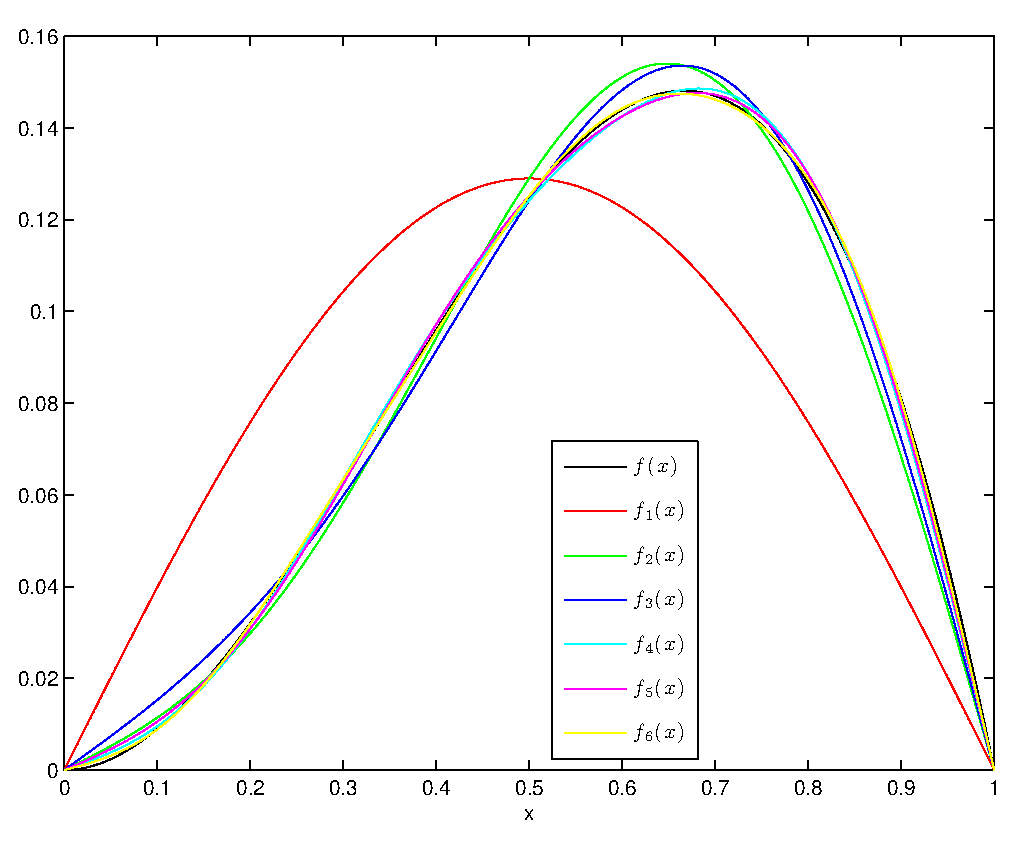
\includegraphics[scale=0.7]{hw27c.eps}\end{center}

The above plot was produced using the following MATLAB code.

\lstinputlisting{HW27c.m}

\item {[2 points]} The requested plot is below.

\begin{center}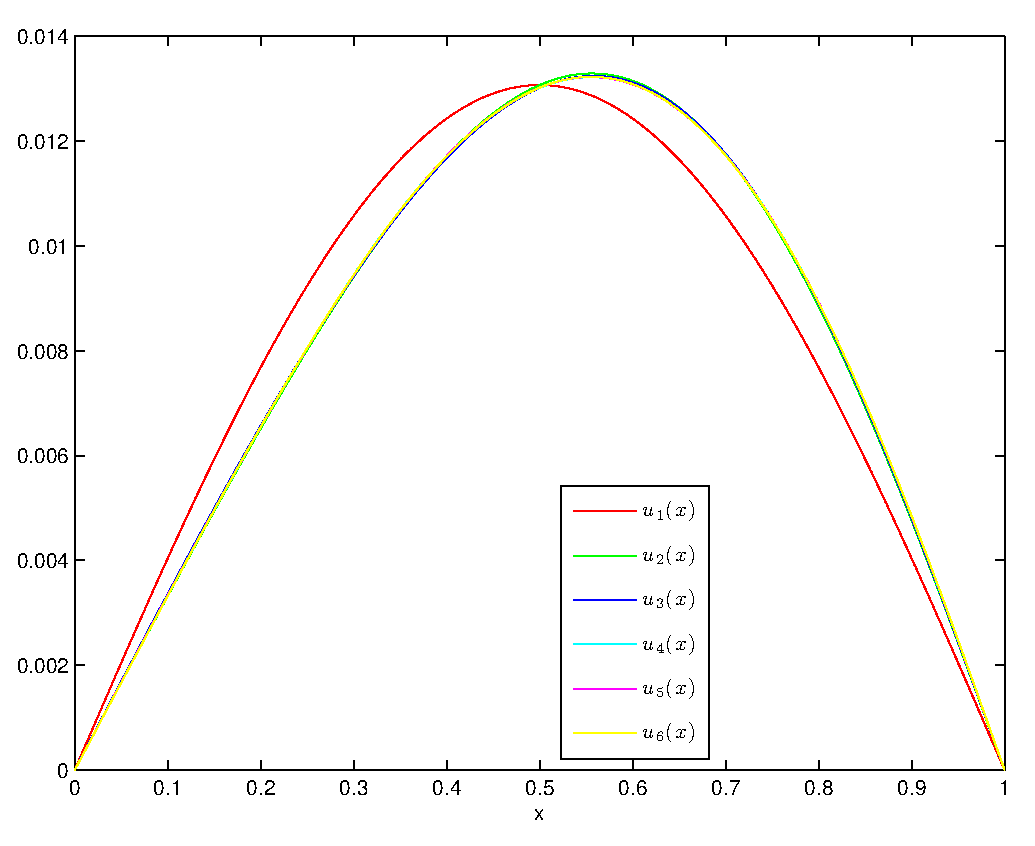
\includegraphics[scale=0.7]{hw27d.eps}\end{center}

The above plot was produced using the following MATLAB code.

\lstinputlisting{HW27d.m}

\item {[2 points]} The series solution that we obtain using the spectral method is
\[
u(x)=\sum_{j=1}^\infty{-4\over j^5\pi^5}\left(1+2\cos\left(j\pi\right)\right)\sin(j\pi x).
\]

\item {[6 points]} Let $u$ be the solution to $Lu=f$ and let $w\in C^2[0,1]$ be such that
\[
-w''(x)=0,\quad0<x<1;
\]
\[
w(0)=-{1\over100}
\]
and
\[
w(1)={1\over100}.
\]
Then $\tilde{u}(x)=w(x)+u(x)$ will be such that
\[
-\tilde{u}''(x)=-w''(x)-u''(x)=0+f(x)=f(x);
\]
\[
\tilde{u}(0)=w(0)+u(0)=-{1\over100}+0=-{1\over100};
\]
and
\[
\tilde{u}(1)=w(1)+u(1)={1\over100}+0={1\over100}.
\]
Now, the general solution to
\[
-w''(x)=0
\]
is $w(x)=Ax+B$ where $A$ and $B$ are constants. Moreover, $w(0)=B$ and so $w(0)=-{1\over100}$ when $B=-{1\over100}$. Hence, $w(x)=Ax-{1\over100}$ and so $w(1)=A-{1\over100}$ and hence $w(1)={1\over100}$ when $A={1\over100}+{1\over100}={2\over100}={1\over50}$. Consequently,
\[
w(x)={1\over50}x-{1\over100}
\]
and so
\[
\tilde{u}(x)={1\over50}x-{1\over100}+u(x).
\]
We can then use the series solution to $Lu=f$ that we obtained in part (e) to obtain the series solution
\[
\tilde{u}(x)={1\over50}x-{1\over100}+\sum_{j=1}^\infty{-4\over j^5\pi^5}\left(1+2\cos\left(j\pi\right)\right)\sin(j\pi x)
\]
to the problem of finding $\tilde{u}\in C^2[0,1]$ such that
\[
-\tilde{u}''(x)=f(x),\quad0<x<1;
\]
\[
\tilde{u}(0)=-{1\over100}
\]
and
\[
\tilde{u}(1)={1\over100}.
\]

\item {[2 points]} The requested plot is below.

\begin{center}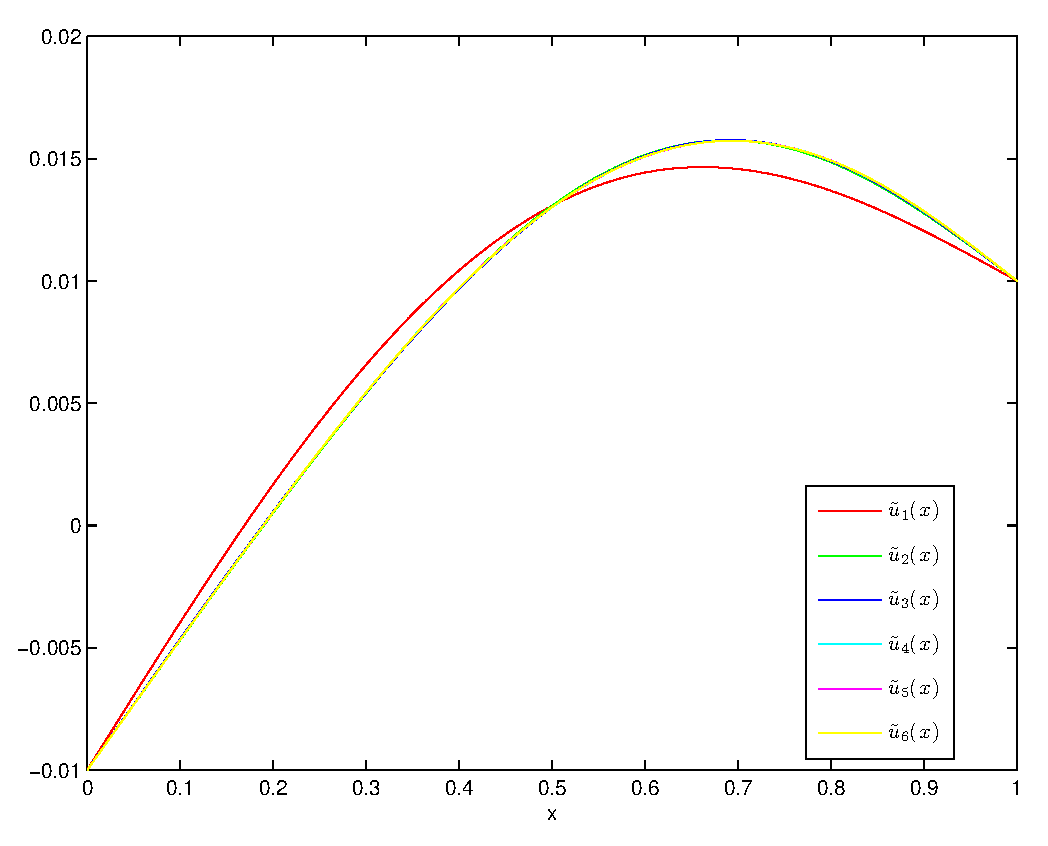
\includegraphics[scale=0.7]{hw27g.eps}\end{center}

The above plot was produced using the following MATLAB code.

\lstinputlisting{HW27g.m}

\end{enumerate}

\end{solution}

